% !TEX TS-program = pdflatex
% !TEX encoding = UTF-8 Unicode

% This is a simple template for a LaTeX document using the "article" class.
% See "book", "report", "letter" for other types of document.

\documentclass[11pt]{article} % use larger type; default would be 10pt

\usepackage[utf8]{inputenc} % set input encoding (not needed with XeLaTeX)

%%% PAGE DIMENSIONS
\usepackage{geometry} % to change the page dimensions
\geometry{a4paper} % or letterpaper (US) or a5paper or....

\usepackage{graphicx} % support the \includegraphics command and options

\usepackage{amssymb}
\usepackage{amsmath}
%%% PACKAGES
\usepackage{booktabs} % for much better looking tables
\usepackage{array} % for better arrays (eg matrices) in maths
\usepackage{paralist} % very flexible & customisable lists (eg. enumerate/itemize, etc.)
\usepackage{verbatim} % adds environment for commenting out blocks of text & for better verbatim
\usepackage{subfig} % make it possible to include more than one captioned figure/table in a single float
% These packages are all incorporated in the memoir class to one degree or another...

%%% HEADERS & FOOTERS
\usepackage{fancyhdr} % This should be set AFTER setting up the page geometry
\pagestyle{fancy} % options: empty , plain , fancy
\renewcommand{\headrulewidth}{0pt} % customise the layout...
\lhead{}\chead{}\rhead{}
\lfoot{}\cfoot{\thepage}\rfoot{}

%%% SECTION TITLE APPEARANCE
\usepackage{sectsty}
\allsectionsfont{\sffamily\mdseries\upshape} % (See the fntguide.pdf for font help)
% (This matches ConTeXt defaults)

%%% ToC (table of contents) APPEARANCE
\usepackage[nottoc,notlof,notlot]{tocbibind} % Put the bibliography in the ToC
\usepackage[titles,subfigure]{tocloft} % Alter the style of the Table of Contents
\renewcommand{\cftsecfont}{\rmfamily\mdseries\upshape}
\renewcommand{\cftsecpagefont}{\rmfamily\mdseries\upshape} % No bold!
\usepackage{graphicx}
\graphicspath{ {./pings/} }

\usepackage{amsmath}
\DeclareMathOperator*{\argmax}{arg\,max}
\DeclareMathOperator*{\argmin}{arg\,min}

\newcount\colveccount
\newcommand*\colvec[1]{
        \global\colveccount#1
        \begin{pmatrix}
        \colvecnext
}
\def\colvecnext#1{
        #1
        \global\advance\colveccount-1
        \ifnum\colveccount>0
                \\
                \expandafter\colvecnext
        \else
                \end{pmatrix}
        \fi
}

%%% END Article customizations

%%% The "real" document content comes below...

\title{Macro PS2}
\author{Michael B. Nattinger\footnote{I worked on this assignment with my study group: Alex von Hafften, Andrew Smith, and Ryan Mather. I have also discussed problem(s) with Emily Case, Sarah Bass, and Danny Edgel.}}

%\date{} % Activate to display a given date or no date (if empty),
         % otherwise the current date is printed 

\begin{document}
\maketitle
\section{Question 1}
We will construct the sequential market structure equilibrium. Each period, we our bond markets contain claims to each "tree". 
\subsection{Part A}
Define $q_t^i$ as the price in period $t$ of a consumption good in period $t+1$ on the condition that consumer $i$ receives an endowment in period $t+1$. $b_t^{i,j}$ is the quantity of that bond demanded by person $j$.

Each agent maximizes expected utility:
\begin{align}
\max_{\{c_t^1,b_t^{1,1},b_t^{2,1}\}_{t=0}^{\infty}} E_0 \sum_{t=0}^{\infty}\beta^tlog c_t^1 \label{eqn:opt1}
\end{align}
\begin{align*}
\text{s.t. } c_t^1 + q_t^1b_t^{1,1} + q_t^2b_t^{2,1} \leq e_t^1 + b_{t-1}^{1,1}1\{ e_t^1=1 \} +  b_{t-1}^{2,1}1\{ e_t^2=1 \} %note: can rewrite indicators as just e from inside the indicator
\end{align*}
\begin{align}
\max_{\{c_t^2,b_t^{1,2},b_t^{2,2}\}_{t=0}^{\infty}} E_0 \sum_{t=0}^{\infty}\beta^tlog c_t^2 \label{eqn:opt2} 
\end{align}
\begin{align*}
\text{s.t. } c_t^2 + q_t^1b_t^{1,2} + q_t^2b_t^{2,2} \leq e_t^2 + b_{t-1}^{1,2}1\{ e_t^1=1 \} +  b_{t-1}^{2,2}1\{ e_t^2=1 \} 
\end{align*}

Market clearing implies the following conditions:
\begin{align}
b_t ^{1,1} + b_t^{1,2} &= 0 \label{eqn:mktcl1} \\
b_t ^{2,1} + b_t^{2,2} &= 0 \label{eqn:mktcl2} \\
c_t^1+c_t^2 &= e_t^1 + e_t^2 \label{eqn:mktcl3}
\end{align}

The competitive equilibrium is a set of prices $\{ q_t^1,q_t^2 \}_{t=0}^{\infty}$ and allocations $\{ b_t^{1,1},b_t^{2,1}, b_t^{1,2},b_t^{2,2},c_t^1,c_t^2\}_{t=0}^{\infty}$ such that agents optimize (\ref{eqn:opt1}),(\ref{eqn:opt2}) and markets clear (\ref{eqn:mktcl1}),(\ref{eqn:mktcl2}),(\ref{eqn:mktcl3}).

\subsection{Part B}
Our bellman equation takes the following form:
%V(b_t^)

Once the future endowment has shifted, it will remain shifted forever. So, 
\subsection{Part C}
\section{Question 2}
\section{Question 3}
\subsection{Part A}
Our bellman equation takes the following form:

\begin{align*}
V(a,l) &= \max_{a'} \frac{(wl +(1+r)a - a')^{1-\gamma}}{1-\gamma} + \beta E[V(a',l')]\\
&=  \max_{a'} \frac{(wl +(1+r)a - a')^{1-\gamma}}{1-\gamma} + \beta (V(a',l_h)P(l'=l_h|l) + V(a',l_h)P(l'=l_h|l))
\end{align*}
Taking FOCs and applying the envelope conditions,
\begin{align*}
(wl +(1+r)a - a')^{-\gamma} &= \beta(V'(a',l_h)P(l'=l_h|l) + V'(a',l_h)P(l'=l_h|l))\\
V'(a,l) &= (1+r)(wl +(1+r)a - a')^{-\gamma}\\
\Rightarrow c^{-\gamma} &= \beta(1+r)((c'_h)^{-\gamma}P(l'=l_h|l) + (c'_l)^{-\gamma}P(l'=l_h|l) )
\end{align*}
The above equation forms our optimality conditions.
\subsection{Part B}
In the stationary distribution, $PQ = P$ where $P = [P_l P_h]$. We can easily solve for this distribution numerically from an arbitrary starting point. As this is a very simple markov process, markov-chain monte carlo methods will converge to the stationary distribution by standard ergodic properties which $Q$ easily satisfies. We can therefore start with an arbitrary initial distribution $P_0$ and iterate through the transition matrix $Q$, with product $P:=P_0Q$ becoming next iteration's $P_0$, until $P$ and $P_0$ have converged to some tolerance. 

The numerical solution is $P = [0.25 0.75] $ so the stationary distribution has $3/4 $ of the weight on the high-labor distribution, and the rest on the low-labor distribution. Therefore, the unconditional mean of the labor endowment is $0.25(0.7) + 0.75(1.1) = 1$.

\subsection{Part C}
I solved for the value function numerically. Results are plotted below.

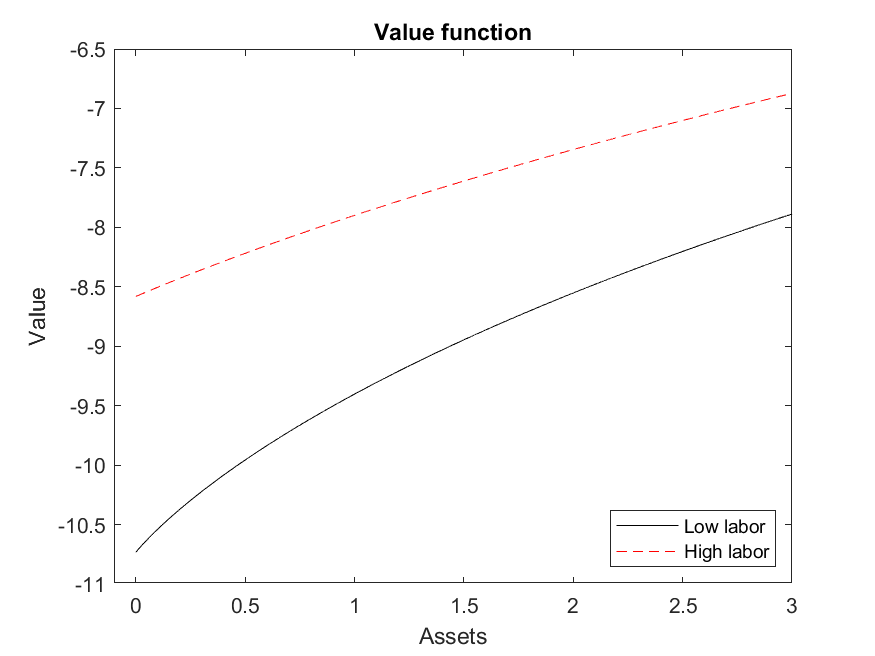
\includegraphics{valfunc}

The value function solution does appear to be continuous, increasing, concave, and differentiable. The value from having a high labor draw is higher than the value from having a low labor draw. All of these features are as predicted by theory.

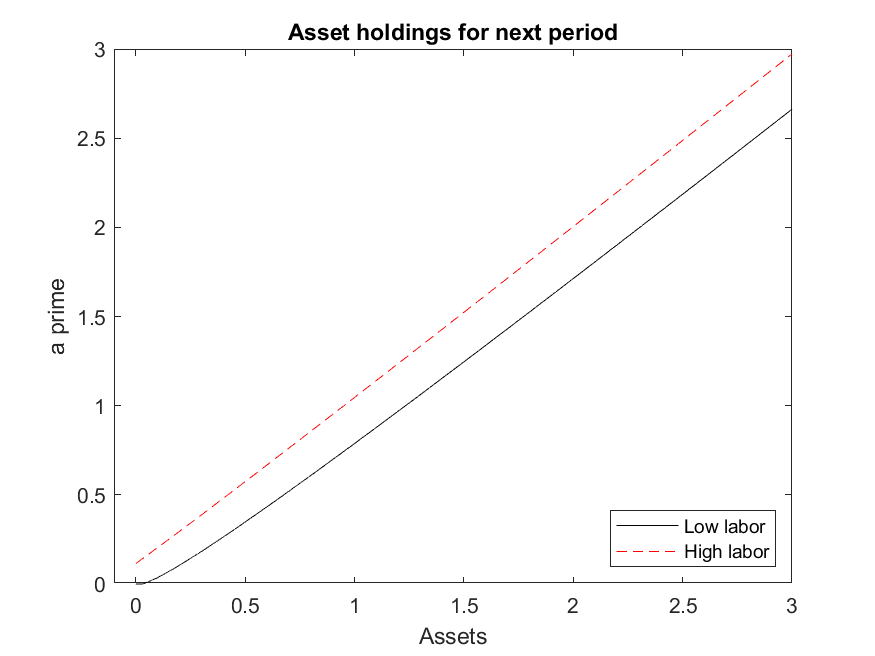
\includegraphics{aprime}


\subsection{Part D}

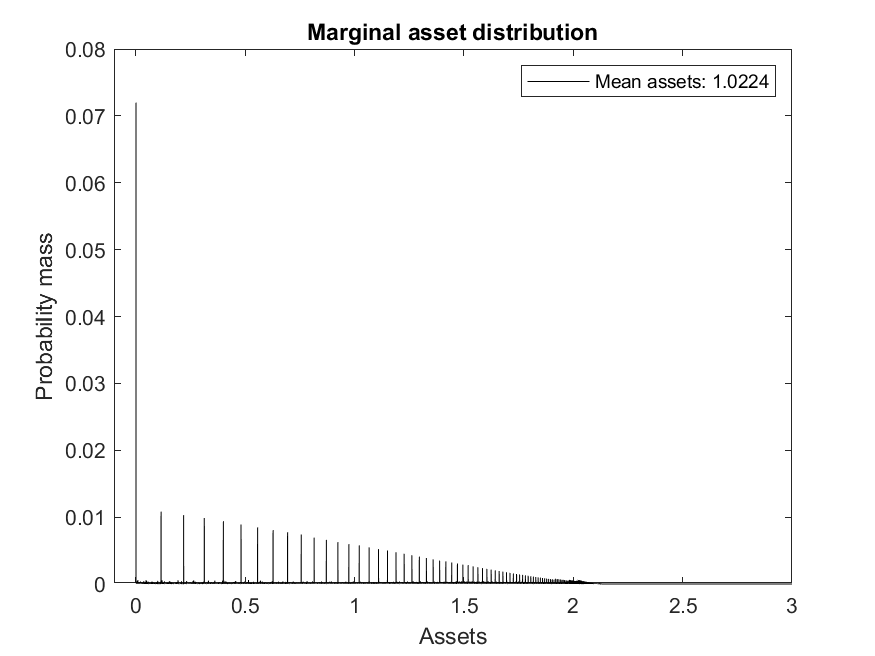
\includegraphics{marginal}
\end{document}
